PMTs were used in TRITIUM experiment with two main objectives. On the one hand, they were used to know the amount of incident photons that reached the PMT photocathode, which can be interesting, for example, to characterize fibers, and, on the other hand, they were used to know the energy of each event detected, which can be interesting, for instance, to obtain an energy spectrum or to discriminate events based on their origin. %(for knowing the origin of these events and counting only interesting events).

In the first case, to know the amount of photons that have reached the photocathode, the PMT should work without the internal gain since it introduces a large uncertainty in the measurement. To do so, the use of the electron multiplication stage (shown in section \ref{subsubsec:PMTs}) must be avoided. It is achieved with a special PCB, shown in Figure \ref{fig:ElectronicSchemeBasePMTNoGain}, which was designed, built and tested.  

%The use of this internal gain could be interesting in other situations such as when we need to know the energy of the event because, as we saw in section \ref{subsubsec:PMTs}, its use greatly enlarges our signal, a factor of the order of $10^6$, and, due to that, it is easier to process and analyze it.

\begin{figure}[htbp]
\centering
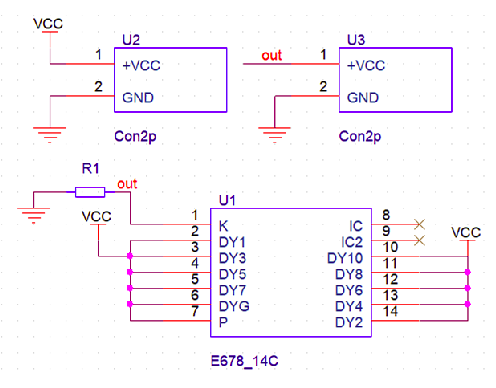
\includegraphics[scale=0.5]{3DesignPrinciples/32Tritium_detector/ElectronicSchemBasePMTNoGain.png}
\caption{Electronic scheme of the electronic voltage divider circuit used for working with PMTs without its internal gain.).\label{fig:ElectronicSchemeBasePMTNoGain}}
\end{figure}

This PCB relies on a short-circuit all the dindes and read the signal directly from the photocathode. It is designed to be powered with positive supply voltage which is less thant the normal situation $[0-400~\volt]$. This is because it is not needed to create a voltage difference between each pair of dynodes in the chain (we only need to create a voltage difference between the photocathode and the first dinode).

Now, the output signal of our photosensor is very small (currents of the order of tens of nanoamperes\footnote{$1~\ampere=10^{9}~\nano\ampere$}) since it is not amplified. Therefore, to analyze these types of currents, a special system is needed. The chosen system is Keithley 6487 Picoammeter/Voltage Source \cite{DataSheetKeithley6487}, which is a commercial system from the Keithley company. It has some interesting options for this study such as automatic baseline correction, the ability to read signals as small as picoamps and the ability to perform some interesting mathematical operation on the signal, such as the average of N measurements with the associated statistical error, where N is programmable by the user ($N=100$ in all our studies).

This is the configuration used to measure the output current of our photosensors. The amount of photons that has reached the photocathode is calculated using the equation \ref{eq:NumPhotonsFromIntensityPMT}:

\begin{equation}
Nº\gamma/\sec = \frac{\left( I_{PMT} - I_{DC} \right)}{q_e \cdot{} QE \cdot{} CE}
\label{eq:NumPhotonsFromIntensityPMT}
\end{equation}

Where $I_{PMT}$ is the output current of the PMT when it detects photons and $I_{DC}$ is the dark current of the PMT. This equation takes into account the quantum efficiency of the PMT used, which is close to $30\%$, and the capture efficiency in the dyndes, which is equal to 1. In addition, it is taken into account that, due to the photoelectric effect in which it consists, each detected photon only generates one electron, the charge of which is $q_e$.

In the second case, to know the energy of the event that occurred, the internal gain of the PMT is needed since it enlarges the signal (usually a factor of the order of $10^6$) which facilitates its processing and analisis. For that the electron multiplication stage shown in section \ref{subsubsec:PMTs} is used.

In all the studies done, the number of PMTs used are one, two or four, depend on the case. A simplified scheme of the electronic chain configurations used in each case is shown in Figures \ref{subfig:ElectronicConfiguraiton1PMT}, \ref{subfig:ElectronicConfiguraiton2PMT} and \ref{subfig:ElectronicConfiguraiton4PMT} respectively, which are based on various NIM technology modules\footnote{The Nuclear Instrumentation Module (NIM) is a standard specification convention for electrical and mechanical parameters defined in electronic modules used in experimental nuclear and particle physics.}.

\begin{figure}[htbp]
 \centering
 \subfloat[Electronical configuraiton scheme used to measure with one PMT.]{
   \label{subfig:ElectronicConfiguraiton1PMT}
    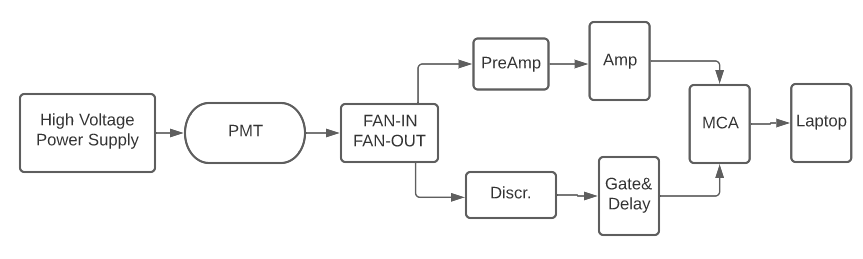
\includegraphics[width=1.0\textwidth]{3DesignPrinciples/32Tritium_detector/Electronical_Scheme_1_PMT.png}}
    \newline  
  \subfloat[Electronical configuraiton scheme used to measure with two PMTs.]{
   \label{subfig:ElectronicConfiguraiton2PMT}
    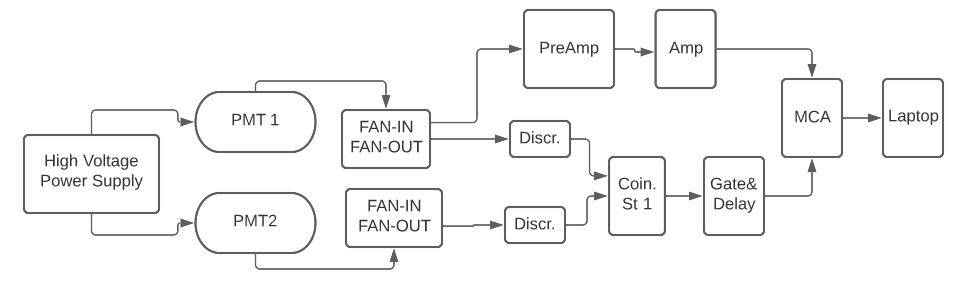
\includegraphics[width=1.0\textwidth]{3DesignPrinciples/32Tritium_detector/Electronical_Scheme_2_PMTs.png}}
    \newline
  \subfloat[Electronical configuraiton scheme used to measure with four PMTs.]{
   \label{subfig:ElectronicConfiguraiton4PMT}
    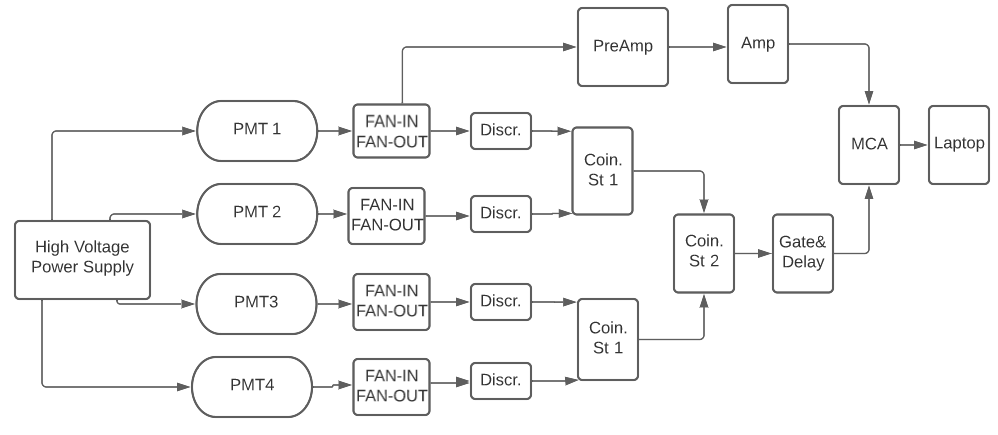
\includegraphics[width=1.0\textwidth]{3DesignPrinciples/32Tritium_detector/Electronical_Scheme_4_PMTs.png}}
 \caption{Schemes of the configuraiton of different electronic chains used to measure with PMTs.}
 \label{fig:ElectronicConfiguraitonsPMT}
\end{figure}

The PMTs used in each situation are feeded with the voltage supply "TC 952 High Voltage Supply" from Tennelec \cite{DataSheetHVSupplyTennelec}. It has four channels for feeding up to four different PMTs. If two or more configurations are needed at the same time, a second voltage supply was used, whose reference is "HV Power Supply N 1130-4" from "Wenzel Elektronik" company \cite{DataSheetHVSupplyWenzel} with 4 additional channels. The high voltage used in each case will be named in the appropriate section.

As can be seen the three Figures, there are two different paths that must be followed by the output signals of each PMT, the amplification part and the time coincidence part. Therefore, the first module needed is an analogic FAN IN-OUT module which is used to duplicate the input signal. The module used is the "Quad linear FAN IN-OUT MODEL 740" module from the company "Philips Scintific" \cite{DataSheetFANINOUT}. It has four different channels and 4 output signals can be obtained from each one, which are identical to the input signal. One of these output signals is used as the input for the amplification part and another is used as the input for the time coincidence part.

\begin{itemize}

\item{} The amplification part, which is the same for all three configurations, is used to process and amplify the output signal. It contains the energy information and is based on two steps:

%We have to take into accout that we have only used the signal from one PMT for the amplification part. We could have added a stage where we add the four PMT output signals and it would probably improve our results, but since our ultimate goal is to work with SiPM, we have not delved into that.

%The electronic path we have followed to achieve this amplification is:

\begin{enumerate}

\item{} One of the output signals of the previous module (FAN IN-OUT) is introduced in a preamplifier, which integrates it, resulting in an output signal the height of which corresponds to the charge of the input pulse. It has a long tail\footnote{The length of the tail is, $\tau=RC$, where R is the input resistance and C is the capacitance used. It is the typical output signal in RC circuits.} due to the use of a capacitance. The preamplifier used is "MODEL 9326 FAST PREAMP" from ORTEC \cite{DataSheetPreAmp}.

\item{} The output signal from the preamplifier is introduced into the amplifier which integer the previous singal. The output singal of it has a shape close to the Gaussian function and it is amplificated by a configured factor. The amplifier modules used are "model 575A" and "model 671", both from ORTEC company \cite{DataSheet575Amp}, \cite{DataSheet671Amp}. An example of the output signal for 575A module is shown in Figure \ref{fig:InputSignalsMCA}, green color.

\end{enumerate}

\item{} The time coincidence part, which  contain the time information. It is used to obtain the coincidence gate that indicates when we have to save the amplified signal (when all the output signals of the used PMTs are in time coincidence). This part has little difference in all three configurations it consists of:

\begin{enumerate}

\item{} One of the output signals of the FAN IN-OUT module of each PMT are introduced into a discriminator module where we obtain an output logic signal with height of $-1.2~\volt$ and width of $240~\nano\second$ when a threshold, the one programmed by the user, is exceeded. The discriminators used in our experiments are  "Octuple Constant-Fraction Discriminator CF8000" module from ORTEC company \cite{DataSheetDiscriminator} and "4 channels discriminator model 84" from CAEN company. 

\item{} Now the time coincidences are made. It is used to ensure that the detected event comes from the scintillating fibers and to remove other events such as external light or dark current events. As it is shown in section \ref{subsec:SetUpActiveShield} and chapter \ref{chap:Prototypes}, each used detectors cointain up two PMTs so time coincidences is done in pairs of photosensors. Due to that, this step is not possible to be applied when only one PMT is used (configuration \ref{subfig:ElectronicConfiguraiton1PMT}). 

Two output logic signals of the discriminator module (which comes from two PMTs that are in the same detector) is connected to a channel of the coincidence module which generate an output signal, with a height of $-1.4~\volt$ and width of $20~\ns$, when both are in time coincidence.

The time coincidence modules used are "Coincidence Unit Model 465" from LeCroy \cite{DataSheetCoincidenceLeCroy} and "Coincidence Type N6234" from CERN-NP \cite{DataSheetCoincidenceCERN}.

\item{} An addition step of time coincidence is included when time coincidence between two different detectors (4 PMTs, configuration \ref{subfig:ElectronicConfiguraiton4PMT} are done. It could be interesting, for exapmle, to detect hard cosmic radiation as we is explained in section \ref{subsec:SetUpActiveShield}.

To do so, a new coincidence step similar to the previous one must be applied. Therefore, two logical output signals of the previous step (coincidence module) are used as input of a second coincidence stage. The output signal of this case has the same parameters, logical signal with a height of $-1.4~\volt$ and width of $20~\nano\second$. The modules used is the same as before.

Some interesting cases  are shown in Figure \ref{fig:DifferentCoincidences} when time coincidences are made in two detectors, 4 PMTs. There, four logical signals are shown, two of them (channel one and two, yellow and green respectively) come from two PMTs connected to one detector and the other two signals (channels three and four, color orange and violet respectively) come from PMTs connected to another detector.

\begin{enumerate}
\item{} In Figure \ref{subfig:signalInOnePMT} only one PMT (channel two) has detected an event. It means that the event detected doesn't come from the scintillator. In this case, the output from coincidence module, stage 1 is not generated and this event is not saved.

\item{} In Figures \ref{subfig:signalInTwoPMTOneDetector} and \ref{subfig:signalInTwoPMTOtherDetector} two PMT signals connected to the same detector have detected an event but the others have not. It means that this event was only detected by one detector. The first coincidence stage will create a output singal but the second not so this event is not saved.

\item{} In Figure \ref{subfig:signalInAllPMTsBothDetector} all signals have detected the event, which means that it is an event that has been detected for both detectors. In this case, a the output signal of both coincidence stage is generated and the event is saved.

\begin{figure}[h]
 \centering
  \subfloat[Event detected in only one PMT.]{
   \label{subfig:signalInOnePMT}
    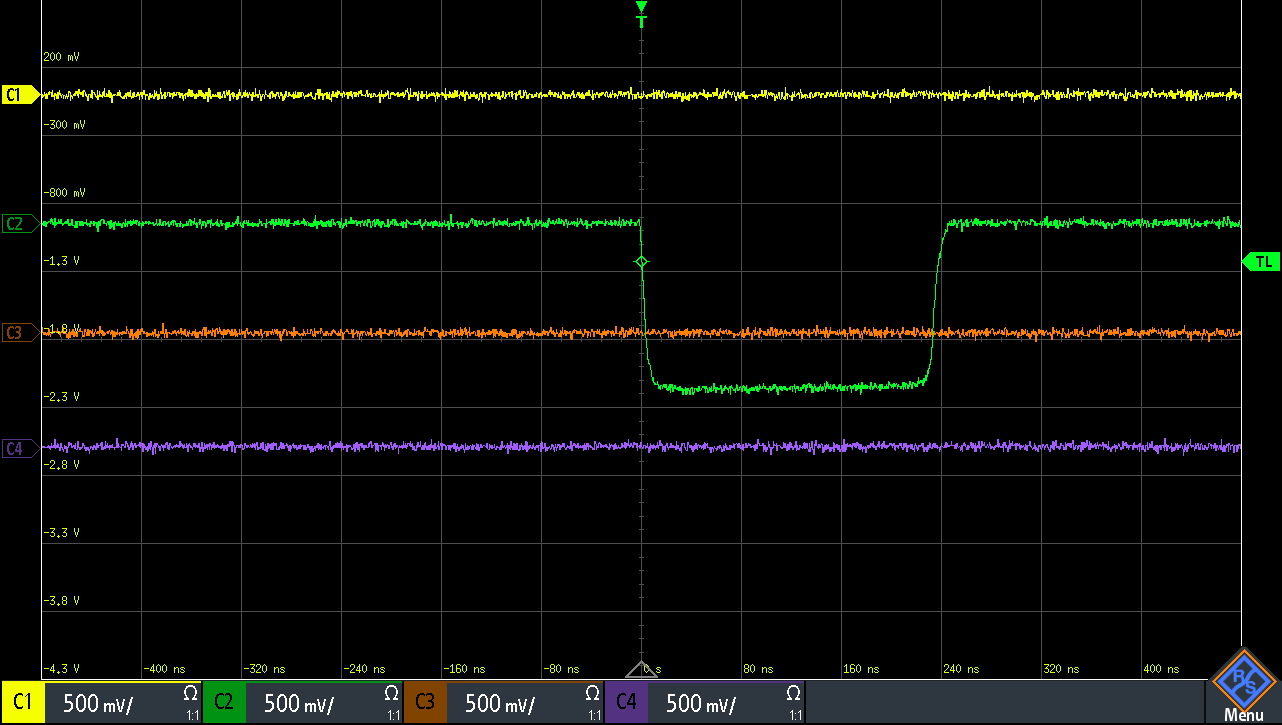
\includegraphics[width=0.5\textwidth]{3DesignPrinciples/32Tritium_detector/1_coincidences.png}}
  \subfloat[Event detected in two PMTs, one detector.]{
   \label{subfig:signalInTwoPMTOneDetector}
    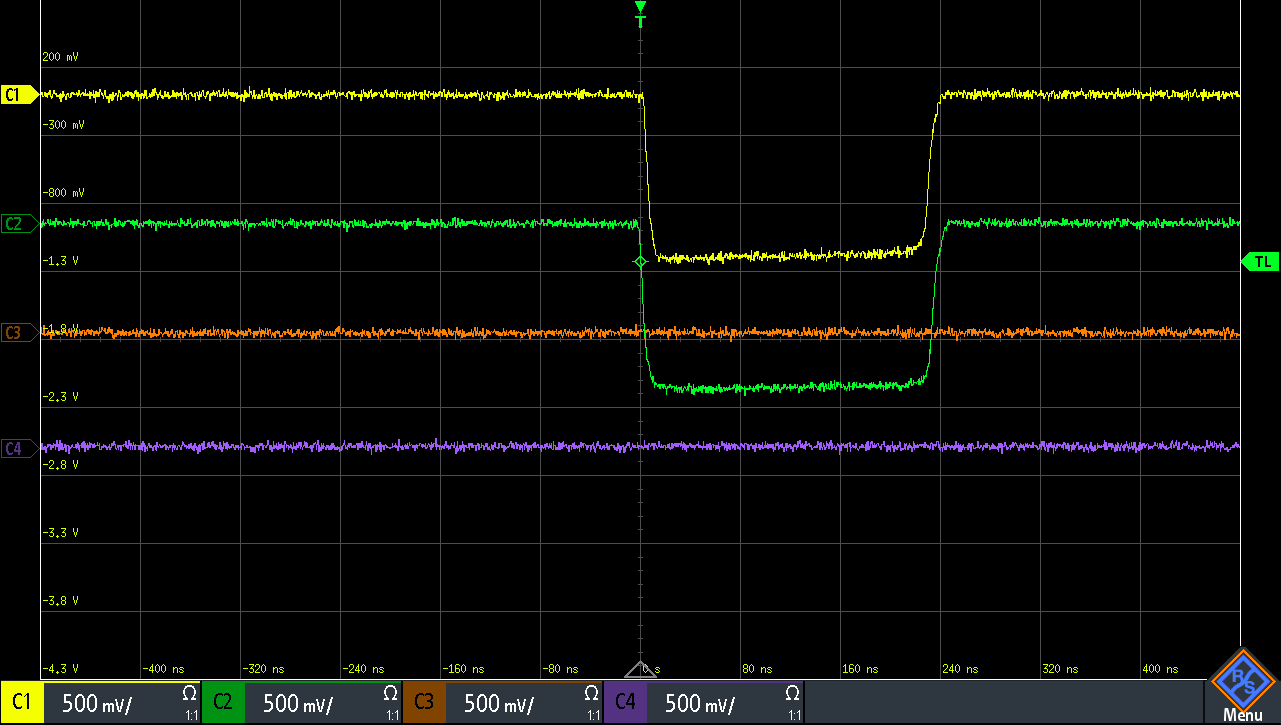
\includegraphics[width=0.5\textwidth]{3DesignPrinciples/32Tritium_detector/2_coincidences_1.png}}
   \newline
  \subfloat[Event detected in two PMTs, other detector.]{
   \label{subfig:signalInTwoPMTOtherDetector}
    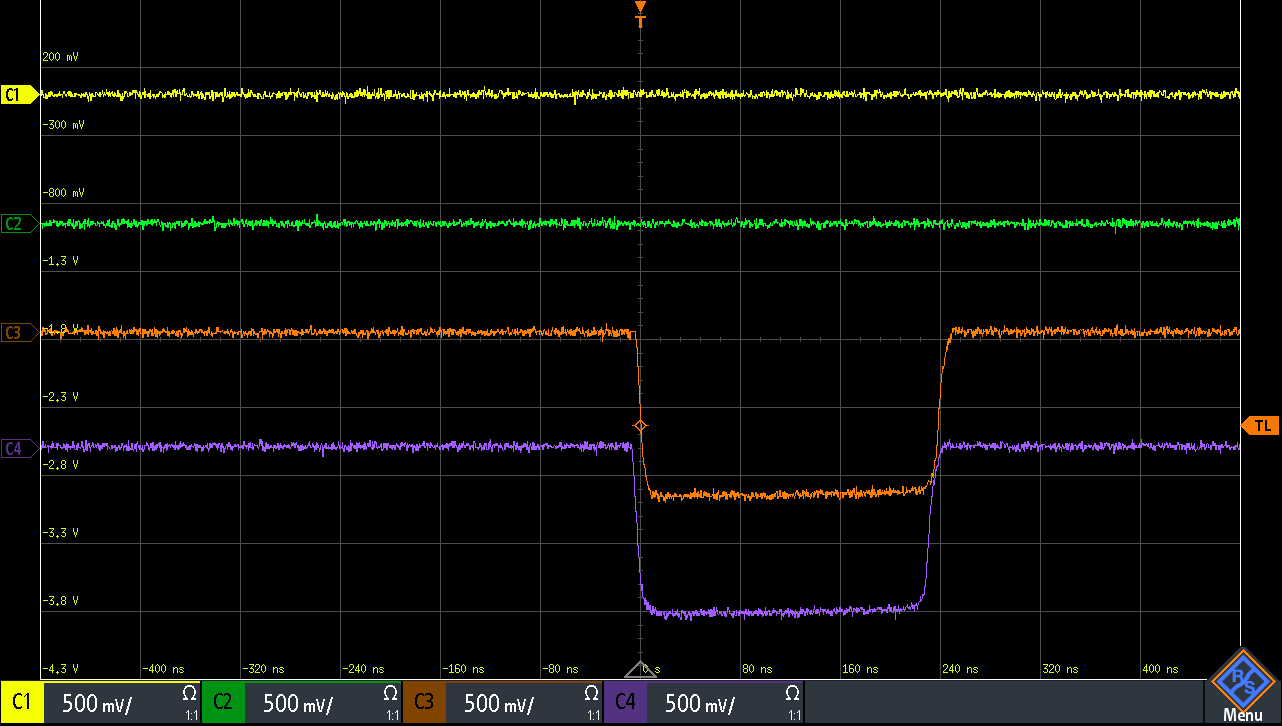
\includegraphics[width=0.5\textwidth]{3DesignPrinciples/32Tritium_detector/2_coincidences_2.png}}
    \subfloat[Event detected in all PMTs, both detector.]{
   \label{subfig:signalInAllPMTsBothDetector}
    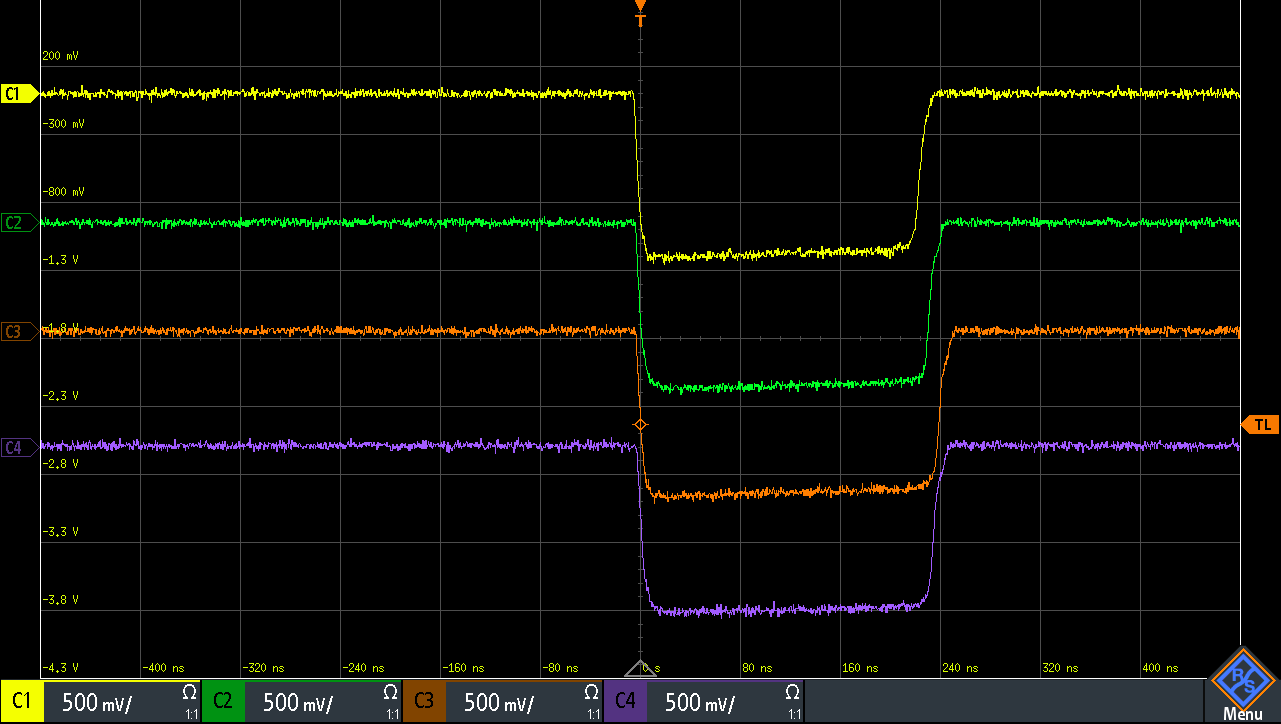
\includegraphics[width=0.5\textwidth]{3DesignPrinciples/32Tritium_detector/4_coincidences.png}}
 \caption{Different situation that can happen when we do time coincidences with PMTs.}
 \label{fig:DifferentCoincidences}
\end{figure}


\end{enumerate}

\item{} Finally, the logical output signal of the last coincidence step, is introduced in the "Gate and Delay Generator", model 416A of the company ORTEC \cite{DataSheetGateAndDelay}. With this NIM module we obtain a positive logical signal, shown in Figure \ref{fig:InputSignalsMCA}, orange color, with a height of $8~\volt$ and width of $2~\mu\second$.

\end{enumerate}

\end{itemize}

At the end, two different output signals are obtained, shown in Figure \ref{fig:InputSignalsMCA}, which will be introduced in the MCA 8000D, Pocket MCA from AMPTEK company \cite{DataSheetMCA} to be saved. On the one hand the analog signal (output from the amplifier module), which has information about the energy of the event and this is the signal whose information we will save for analyzing. On the other hand the logic signal (output from the Gate and Delay Generator module) that indicates when the amplified signal must be saved.

\begin{figure}[htbp]
\centering
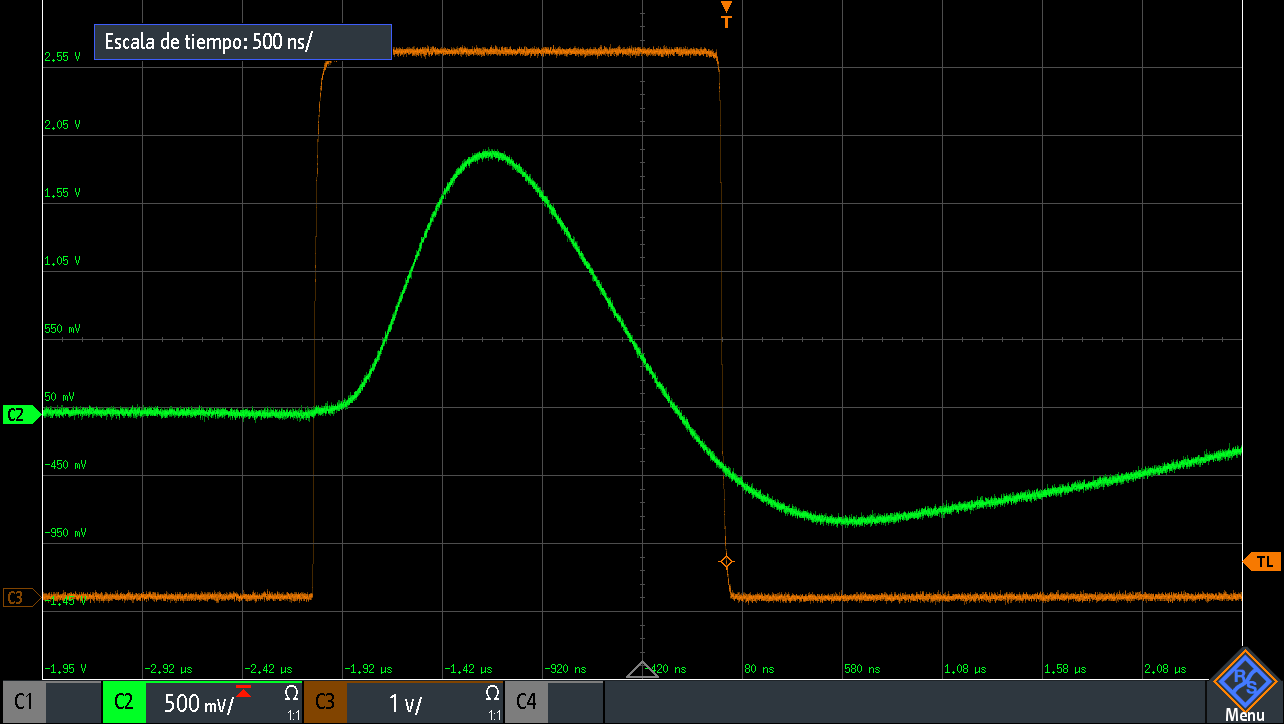
\includegraphics[scale=0.3]{3DesignPrinciples/32Tritium_detector/Input_MCA.png}
\caption{Signal amplificated and logical gate (input signals of MCA).\label{fig:InputSignalsMCA}}
\end{figure}

The MCA is a module used to save the signal information as a histogram. The histogrammed variable is the height of the input pulse of the signal (green signal), which, in the case of the electronic configuration used, corresonds corresponds to the energy of the event. It is performed when the value of the signal gate (orange signal) is greater than $4~\volt$, which indicate that it is an interesting event.

%An example of histogram as output of the MCA is shown in figure \ref{fig:EnergySpectrum4PMTs}.

%\begin{figure}[htbp]
%\centering
%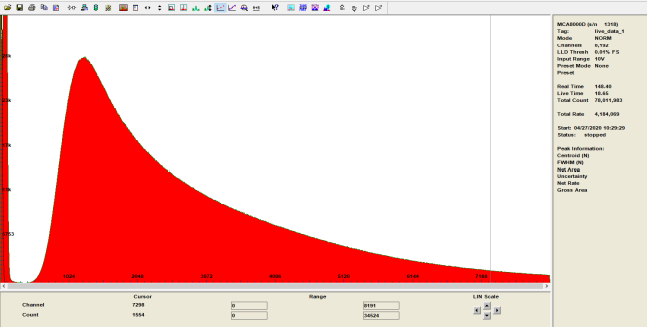
\includegraphics[scale=0.6]{3DesignPrinciples/32Tritium_detector/EspectroEnergeticoMCA.png}
%\caption{Energy spectrum obtained with the electronic configuration explained in this section for four PMTs.\label{fig:EnergySpectrum4PMTs}}
%\end{figure}
